\section{Schaltung}
\label{sec:Schaltung}

%Schaltung zeigen
%Funktionsweise der Schaltung
%Welche Tests sinnvoll und warum

In der Bachelor-Thesis von Simon Hasler ist eine Teilschaltung implementiert, welche den Strom eines Asynchronmotors misst. Diese Schaltung wurde von den Autoren ausgewählt, um im Modul EMV Tests durchführen zu können. Damit die Schaltung bei den Tests sicher nicht kaputt geht, sollte diese nachgebaut werden. Leider wurde bekannt, dass diese Teilschaltung, generiert von einer anderen, externen Schule, nicht funktionstüchtig ist. Aus diesem Grund haben die Autoren eine eigene Schaltung zur Strommessung mit an der Fachhochschule zur Verfügung stehenden Mitteln zusammengestellt. Bei der Schaltung handelt es sich um eine Strommessung über einen Widerstand (Shunt) mit Tiefpassfilterung und einem Operationsverstärker, zu sehen in Abbildung \ref{fig:Schaltung}.

\begin{minipage}[b][6cm][t]{1\textwidth}
\centering
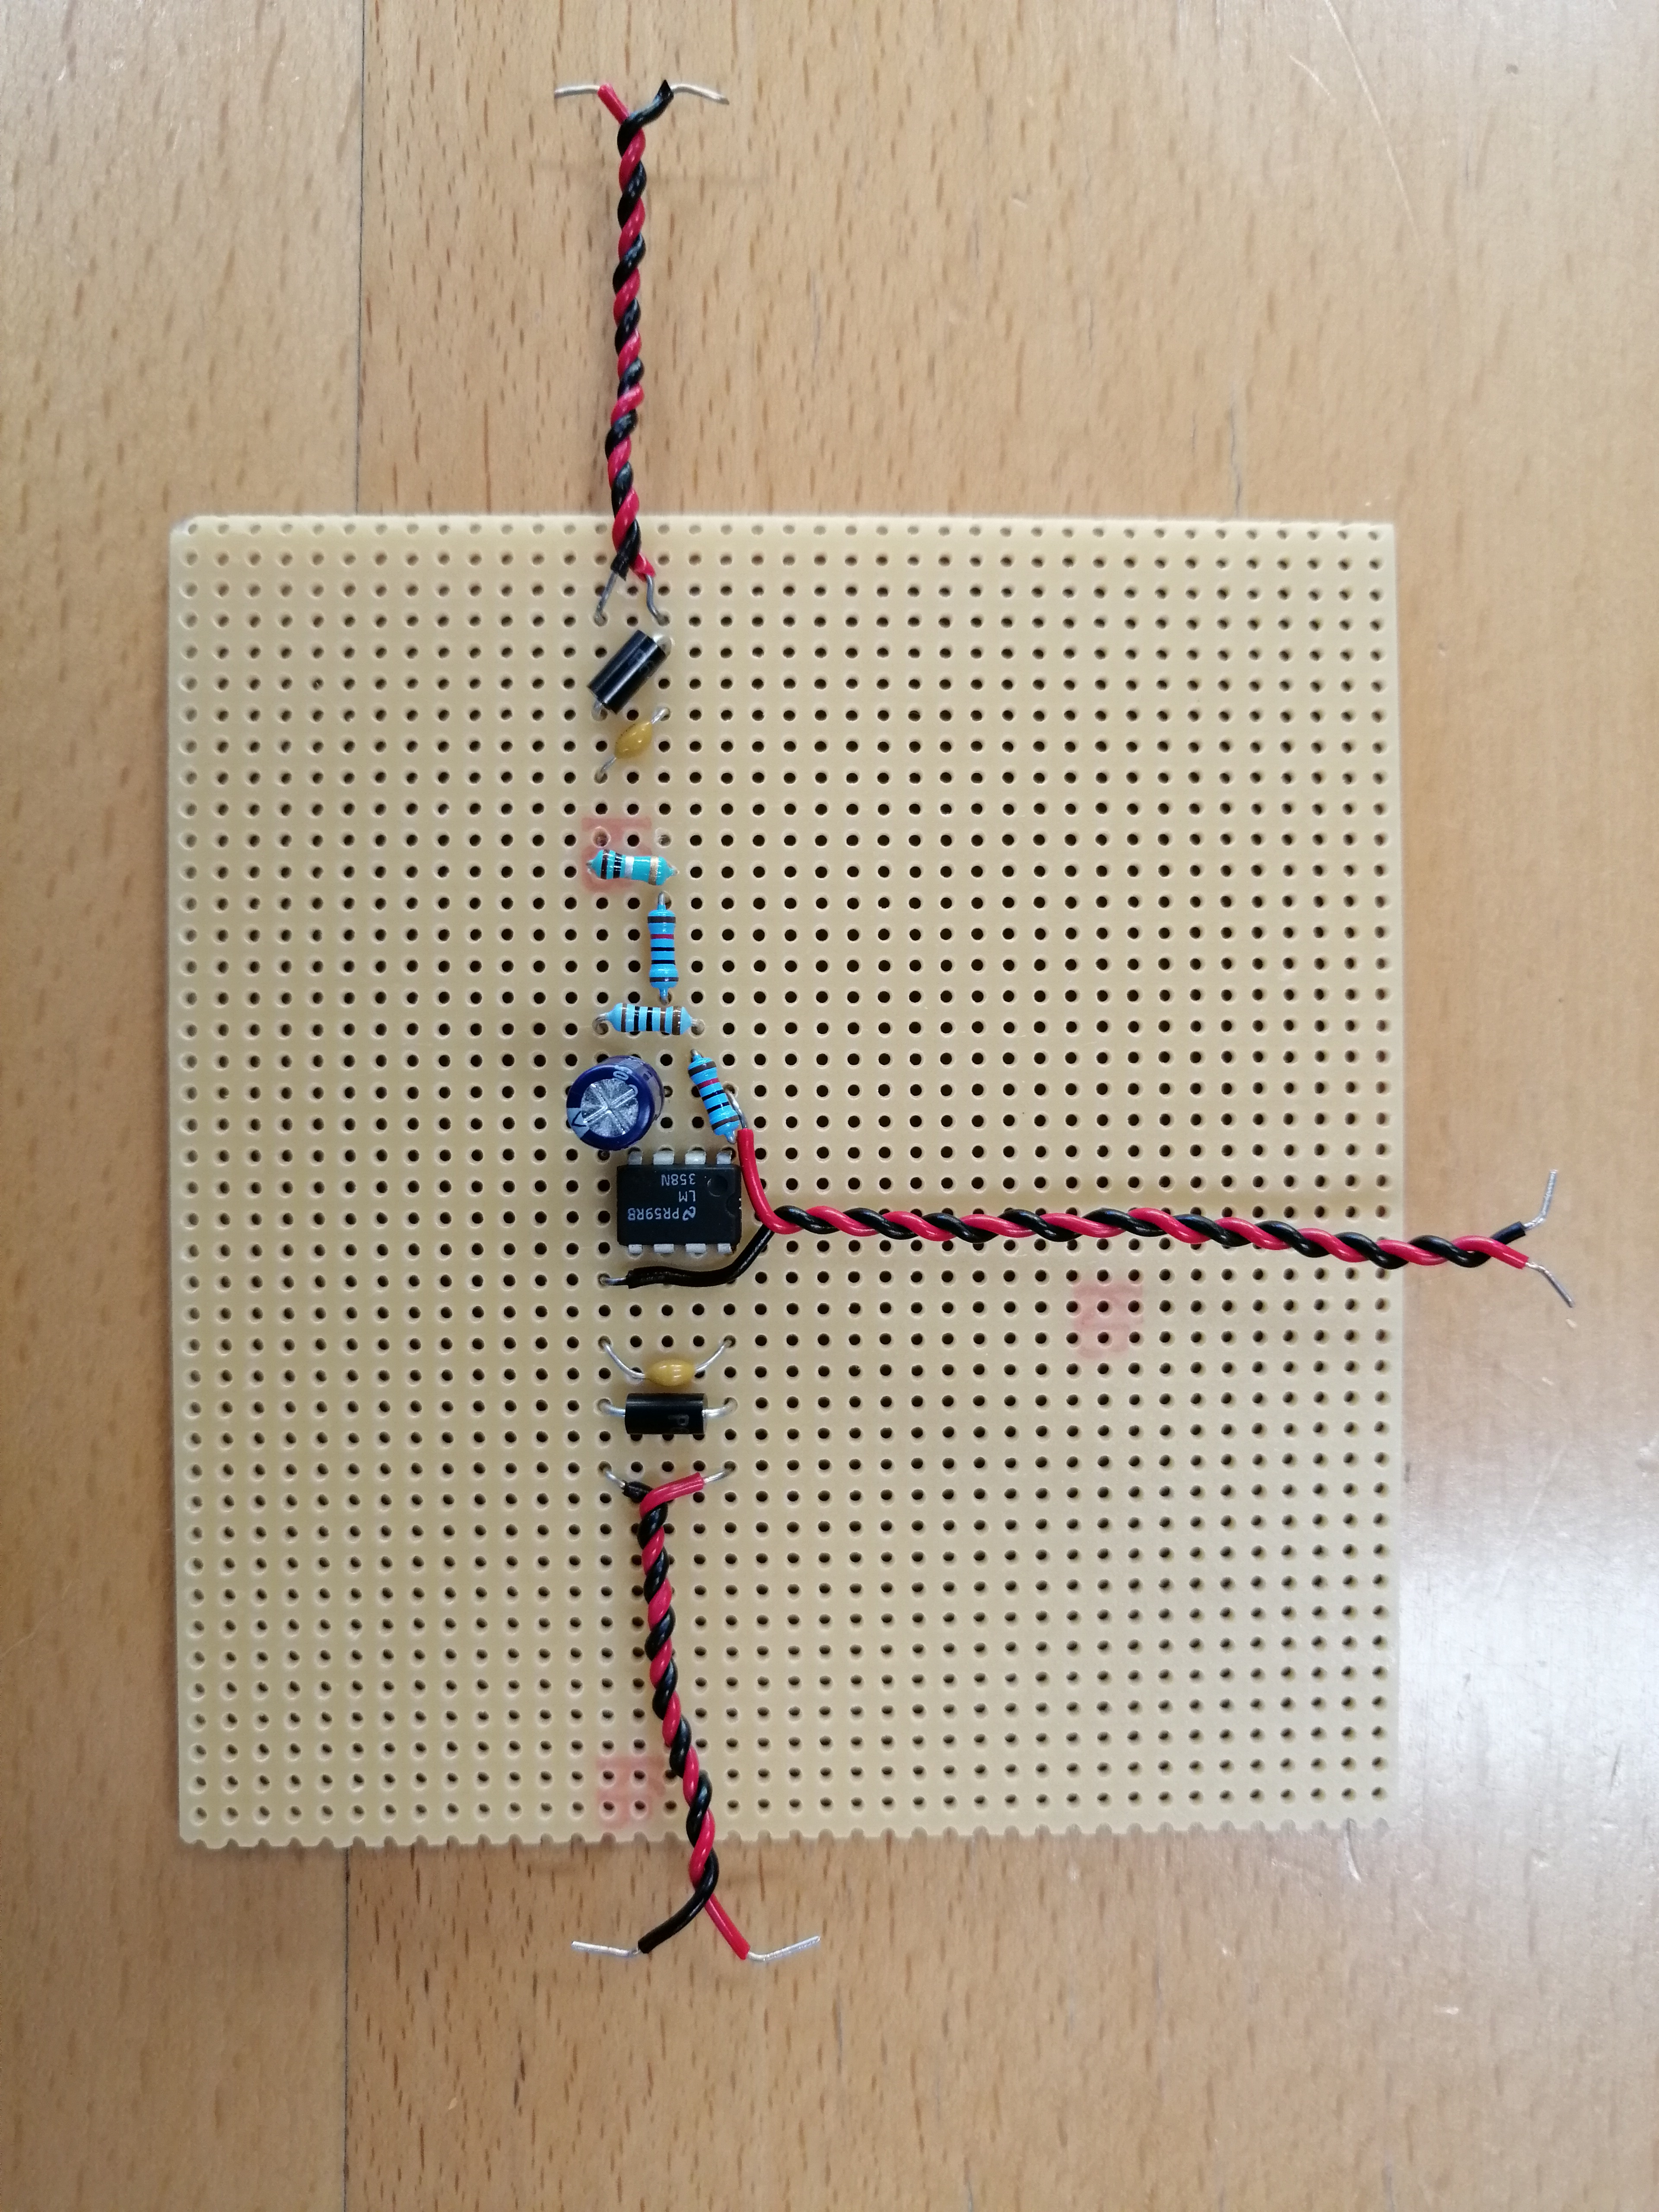
\includegraphics[angle=90,width=0.75\textwidth]{graphics/Schaltung.jpg}
\captionof{figure}{Die entworfene Schaltung zur Strommessung.}
\label{fig:Schaltung}
\end{minipage}

